\documentclass[11pt]{article}

% ====================================================
% PACKAGES
% ====================================================
\usepackage[margin=1in, headheight=13.6pt]{geometry}
\usepackage[T1]{fontenc}
\usepackage{lmodern}
\usepackage{microtype}
\usepackage{setspace}
\usepackage{tcolorbox}
\usepackage{amsmath, amssymb, mathtools}
\usepackage{siunitx}
\usepackage{bm}

\usepackage{graphicx}
\usepackage{float}
\usepackage{subcaption}

\usepackage{enumitem}
\usepackage{booktabs}
\usepackage{longtable}
\usepackage{array}
\usepackage{multirow}

\usepackage{xcolor}
\usepackage{hyperref}

\usepackage{fancyhdr}
\usepackage{lastpage}

\usepackage{indentfirst}
\usepackage[justification=centering]{caption}
\usepackage{pdfpages}
\usepackage{listings}

\lstdefinestyle{pystyle}{
    language=Python,
    basicstyle=\ttfamily\small,
    keywordstyle=\color{blue!60!black}\bfseries,
    commentstyle=\color{green!40!black}\itshape,
    stringstyle=\color{orange!70!black},
    numbers=left,
    numberstyle=\tiny\color{gray},
    numbersep=6pt,
    breaklines=true,
    breakatwhitespace=false,
    showstringspaces=false,
    frame=single,
    rulecolor=\color{gray!50},
    tabsize=4
}
\lstset{style=pystyle}

\pagestyle{fancy}
\fancyhf{}
\lhead{\Assignment\ |\ \course}
\rhead{\Name\ |\ \today}
\cfoot{Page \thepage\ of~\pageref{LastPage}}

\hypersetup{
    colorlinks,
    linkcolor={red!50!black},
    citecolor={blue!50!black},
    urlcolor={blue!80!black}
}

\newcommand{\Name}{Arael Anaya}
\newcommand{\Assignment}{Homework 7}
\newcommand{\course}{Robot Mechanics}

% Boxed final-answer environment
\newtcolorbox{result}{
    colback=blue!3!white,
    colframe=blue!40!black,
    boxrule=0.6pt,
    arc=2pt,
    left=6pt, right=6pt, top=4pt, bottom=4pt
}

% Boxed problem-statement environment
\newtcolorbox{statement}{
    colback=gray!5!white,
    colframe=gray!50!black,
    boxrule=0.4pt,
    arc=2pt,
    left=6pt, right=6pt, top=4pt, bottom=4pt
}

% Visible placeholder for work not yet added
\newcommand{\workplaceholder}{%
    \par\vspace{4pt}\noindent\textcolor{gray!60}{\itshape [Work not yet added: paste solution here]}\par\vspace{4pt}%
}

% Boxed correction-note environment (flags a fix made to the original hand calc)
\newtcolorbox{fixnote}{
    colback=orange!5!white,
    colframe=orange!55!black,
    boxrule=0.5pt,
    arc=2pt,
    left=6pt, right=6pt, top=4pt, bottom=4pt,
    fontupper=\small
}

% Notation macros (matching course conventions)
\newcommand{\T}{\bm{T}}
\newcommand{\R}{\bm{R}}
\newcommand{\dvec}{\bm{d}}
\newcommand{\framen}[1]{\{#1\}}
\newcommand{\khat}{\widehat{\bm{k}}}
\newcommand{\wvec}{\bm{\omega}}
\newcommand{\xivec}{\bm{\xi}}
\newcommand{\vvec}{\bm{v}}
\newcommand{\Omvec}{\bm{\Omega}}
\newcommand{\Rotx}{\operatorname{Rot}_x}
\newcommand{\Roty}{\operatorname{Rot}_y}
\newcommand{\Rotz}{\operatorname{Rot}_z}
\newcommand{\atantwo}{\operatorname{atan2}}
\newcommand{\skewx}[1]{\left[#1\right]_{\times}}

\begin{document}

% ====================================================
% PROBLEM 1
% ====================================================
\section*{Problem 1}

\begin{statement}
Calculate the time derivative of the following rotation matrices. The angular velocity $\wvec$ is expressed in the fixed frame.
\begin{enumerate}[label=(\alph*), nosep]
\item $\wvec=\begin{bmatrix}0\\0\\1\end{bmatrix}\,\mathrm{rad/s},\quad \R=\begin{bmatrix}0.5&-0.866&0\\0.866&0.5&0\\0&0&1\end{bmatrix}.$
\item $\wvec=\begin{bmatrix}0\\1\\0\end{bmatrix}\,\mathrm{rad/s},\quad \R=\begin{bmatrix}0.5&-0.866&0\\0.866&0.5&0\\0&0&1\end{bmatrix}.$
\item $\wvec=\begin{bmatrix}1\\0\\0\end{bmatrix}\,\mathrm{rad/s},\quad \R=\begin{bmatrix}0.5&-0.866&0\\0.866&0.5&0\\0&0&1\end{bmatrix}.$
\item $\wvec=\begin{bmatrix}0.91340\\0.63240\\0.09754\end{bmatrix}\,\mathrm{rad/s},\quad \R=\begin{bmatrix}-0.62170&-0.02073&-0.78300\\-0.13850&-0.98100&0.13590\\-0.77090&0.19300&0.60700\end{bmatrix}.$
\end{enumerate}
\end{statement}

\textbf{Solution.} With the angular velocity expressed in the fixed frame, $\dot{\R}=\skewx{\wvec}\R$.
\begin{enumerate}[label=(\alph*), nosep]
\item $\dot{\R}=\begin{bmatrix}-0.866&-0.5&0\\0.5&-0.866&0\\0&0&0\end{bmatrix}$
\item $\dot{\R}=\begin{bmatrix}0&0&1\\0&0&0\\-0.5&0.866&0\end{bmatrix}$
\item $\dot{\R}=\begin{bmatrix}0&0&0\\0&0&-1\\0.866&0.5&0\end{bmatrix}$
\item $\dot{\R}=\begin{bmatrix}-0.474&0.218&0.371\\0.643&-0.178&-0.631\\0.267&-0.883&0.619\end{bmatrix}$
\end{enumerate}

\bigskip
% ====================================================
% PROBLEM 2
% ====================================================
\section*{Problem 2}

\begin{statement}
A quadcopter is flying around with an inertial measurement unit (IMU) attached $10\,$cm offset from the center of mass (Figure~\ref{fig:drone}). An external observer measures the position, orientation, linear and angular velocity, and linear acceleration of the quadcopter relative to a fixed ground reference system (origin $0$). What is the linear velocity and acceleration, and angular velocity measured by the IMU in the body frame of the quadcopter at this instant? The angular velocity remains constant. \emph{Hint: Do not forget gravity.}
\[
{}^0\dvec_{01}=\begin{bmatrix}20\\15\\10\end{bmatrix}\mathrm{m},\quad
{}^0\R_1=\begin{bmatrix}0.5&-0.866&0\\0.866&0.5&0\\0&0&1\end{bmatrix},\quad
{}^0\vvec_{01}=\begin{bmatrix}10\\5\\0.25\end{bmatrix}\mathrm{m/s},
\]
\[
{}^0\bm{a}_{01}=\begin{bmatrix}-1\\0\\0.1\end{bmatrix}\mathrm{m/s}^2,\quad
{}^0\wvec_{01}=\begin{bmatrix}0\\0\\2.3\end{bmatrix}\mathrm{rad/s}.
\]
\end{statement}

\begin{figure}[H]
    \centering
    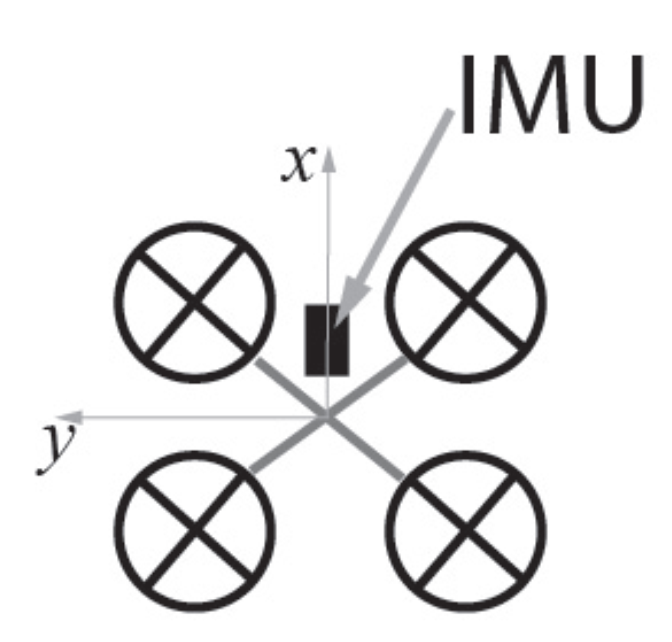
\includegraphics[width=.25\columnwidth]{Figures/drone_imu.png}
    \caption{IMU offset from the center of mass.}
    \label{fig:drone}
\end{figure}

\textbf{Solution.} The IMU offset in the body frame is ${}^1\bm{r}_{\mathrm{imu}}=[0.1\ \ 0\ \ 0]^{\intercal}$\,m. Since $\wvec$ is constant, $\dot{\wvec}=\bm{0}$, so
\[
\vvec_P=\vvec_{\mathrm{com}}+\wvec\times\bm{r},\qquad
\bm{a}_P=\bm{a}_{\mathrm{com}}+\wvec\times(\wvec\times\bm{r}).
\]
Offset in the fixed frame:
\[
{}^0\bm{r}_{\mathrm{imu}}={}^0\R_1\,{}^1\bm{r}_{\mathrm{imu}}=\begin{bmatrix}0.05\\0.0866\\0\end{bmatrix}\mathrm{m}.
\]
Velocity:
\[
{}^0\vvec_{\mathrm{imu}}={}^0\vvec_{01}+{}^0\wvec_{01}\times{}^0\bm{r}_{\mathrm{imu}}=\begin{bmatrix}9.8008\\5.115\\0.25\end{bmatrix}\mathrm{m/s},\qquad
{}^1\vvec_{\mathrm{imu}}={}^0\R_1^{\intercal}\,{}^0\vvec_{\mathrm{imu}}.
\]
Acceleration (gravity ${}^0\bm{g}=[0\ \ 0\ \ {-9.81}]^{\intercal}$\,m/s$^2$ is subtracted, since an IMU measures specific force):
\[
{}^0\bm{a}_{\mathrm{imu}}={}^0\bm{a}_{01}+\skewx{{}^0\wvec_{01}}\skewx{{}^0\wvec_{01}}\,{}^0\bm{r}_{\mathrm{imu}}=\begin{bmatrix}-1.2645\\-0.458\\0.1\end{bmatrix},\qquad
{}^1\bm{a}_{\mathrm{meas}}={}^0\R_1^{\intercal}\left({}^0\bm{a}_{\mathrm{imu}}-{}^0\bm{g}\right).
\]
\begin{result}
\[
{}^1\vvec_{\mathrm{imu}}=\begin{bmatrix}9.33\\-5.93\\0.25\end{bmatrix}\mathrm{m/s},\quad
{}^1\bm{a}_{\mathrm{meas}}=\begin{bmatrix}-1.029\\0.866\\9.91\end{bmatrix}\mathrm{m/s}^2,\quad
{}^1\wvec_{01}={}^0\R_1^{\intercal}\,{}^0\wvec_{01}=\begin{bmatrix}0\\0\\2.3\end{bmatrix}\mathrm{rad/s}
\]
\end{result}
% \begin{fixnote}
% \textbf{Correction to the hand calculation.} The hand calc used ${}^0a_{01,z}=1\,\mathrm{m/s^2}$, but the problem statement gives $0.1\,\mathrm{m/s^2}$. This changes the $z$-component of the measured acceleration from $10.81$ to $9.91\,\mathrm{m/s^2}$. The $x$ and $y$ components are unaffected. The result above uses the value from the problem statement.
% \end{fixnote}

\bigskip
% ====================================================
% PROBLEM 3
% ====================================================
\section*{Problem 3}

\begin{statement}
Consider a three-link manipulator with joint angles $\bm{\theta}=[\pi/3\ \ \pi/6\ \ \pi/6]^{\intercal}$\,rad, joint angle rates $\dot{\bm{\theta}}=[0.5\ \ {-1.0}\ \ 1.5]^{\intercal}$\,rad/s, a stationary base, and the following DH table. Assume that the angle rates remain constant. What are the angular velocities $\wvec_i$, linear velocities $\dot{\dvec}_{0,i}$, and accelerations $\ddot{\dvec}_{0,i}$ at each frame (i.e., $i=1,2,3$)? In addition, construct the velocity Jacobian. \emph{Hint: The velocity of the end frame is} $\bm{J}_{\mathrm{v}}\dot{\bm{\theta}}=[-0.1924\ \ 0.2498\ \ {-0.3580}\ \ 0.4330\ \ {-0.2500}\ \ 0.5000]^{\intercal}$.
\begin{center}
\begin{tabular}{c|cccc}
Link & $a$ & $d$ & $\alpha$ & $\theta$ \\ \hline
1 & $0$ & $1$ & $\pi/2$ & $\star$ \\
2 & $0.5$ & $0$ & $0$ & $\star$ \\
3 & $0.3$ & $0$ & $0$ & $\star$
\end{tabular}
\end{center}
\end{statement}

\textbf{Solution.} Build each link transform from the standard DH form
\[
\bm{A}_i=\begin{bmatrix}
c_{\theta}&-s_{\theta}c_{\alpha}&s_{\theta}s_{\alpha}&a\,c_{\theta}\\
s_{\theta}&c_{\theta}c_{\alpha}&-c_{\theta}s_{\alpha}&a\,s_{\theta}\\
0&s_{\alpha}&c_{\alpha}&d\\
0&0&0&1
\end{bmatrix},\qquad
{}^0\T_i=\prod_{k=1}^{i}\bm{A}_k,
\]
and read off the origins $\dvec_{0,i}$ and axes $\bm{z}_i$ (third column of ${}^0\R_i$), all in frame $\framen{0}$. All joints are revolute and the base is stationary ($\wvec_0=\dot{\dvec}_{0,0}=\bm{0}$), so with $\bm{r}_i=\dvec_{0,i}-\dvec_{0,i-1}$ propagate outward for $i=1,2,3$:
\begin{align*}
\wvec_i&=\wvec_{i-1}+\dot\theta_i\,\bm{z}_{i-1},\\
\dot{\wvec}_i&=\dot{\wvec}_{i-1}+\ddot\theta_i\,\bm{z}_{i-1}+\dot\theta_i\,\wvec_{i-1}\times\bm{z}_{i-1}\quad(\ddot\theta_i=0),\\
\dot{\dvec}_{0,i}&=\dot{\dvec}_{0,i-1}+\wvec_i\times\bm{r}_i,\\
\ddot{\dvec}_{0,i}&=\ddot{\dvec}_{0,i-1}+\dot{\wvec}_i\times\bm{r}_i+\wvec_i\times(\wvec_i\times\bm{r}_i).
\end{align*}
The Jacobian columns are
\[
\bm{J}_i=\begin{bmatrix}\bm{z}_{i-1}\times(\dvec_{0,3}-\dvec_{0,i-1})\\ \bm{z}_{i-1}\end{bmatrix},\qquad
\begin{bmatrix}\dot{\dvec}_{0,3}\\ \wvec_3\end{bmatrix}=\bm{J}\dot{\bm{\theta}}.
\]
Evaluating in MATLAB (Appendix~A):
\begin{center}
\small
\begin{tabular}{c|ccc}
Frame $i$ & $\wvec_i$ (rad/s) & $\dot{\dvec}_{0,i}$ (m/s) & $\ddot{\dvec}_{0,i}$ (m/s$^2$) \\ \hline
1 & $[0,\ 0,\ 0.5]$ & $[0,\ 0,\ 0]$ & $[0,\ 0,\ 0]$ \\
2 & $[-0.8660,\ 0.5,\ 0.5]$ & $[-0.0625,\ 0.3248,\ -0.4330]$ & $[-0.4871,\ -0.3438,\ -0.2500]$ \\
3 & $[0.4330,\ -0.2500,\ 0.5]$ & $[-0.1924,\ 0.2498,\ -0.3580]$ & $[-0.4121,\ -0.4737,\ -0.3150]$
\end{tabular}
\end{center}
\begin{result}
\[
\bm{J}=\begin{bmatrix}
-0.5049&-0.2549&-0.1299\\
0.2915&-0.4415&-0.2250\\
0&0.5830&0.1500\\
0&0.8660&0.8660\\
0&-0.5000&-0.5000\\
1&0&0
\end{bmatrix},\qquad
\bm{J}\dot{\bm{\theta}}=\begin{bmatrix}-0.1924\\0.2498\\-0.3580\\0.4330\\-0.2500\\0.5000\end{bmatrix}
\]
\end{result}
\bigskip
% ====================================================
% APPENDIX A: CODE
% ====================================================
\newpage
\section*{Appendix A: Code}

% Listings are skipped until the code file exists, so a missing file cannot break the build.
\newcommand{\codelisting}[2]{%
    \IfFileExists{../Code/#1}{\lstinputlisting[language=#2, caption={\detokenize{#1}}]{"../Code/#1"}}%
    {\noindent\textcolor{gray!60}{\itshape [#1 not yet written]}}%
}

\subsection*{Problem3.m}\codelisting{Problem3.m}{Matlab}

% ====================================================
% APPENDIX B: HAND CALCULATIONS
% ====================================================
\newpage
\section*{Appendix B: Hand Calculations}\label{app:hand}

\IfFileExists{../Homework_7_hand_calcs.pdf}{%
    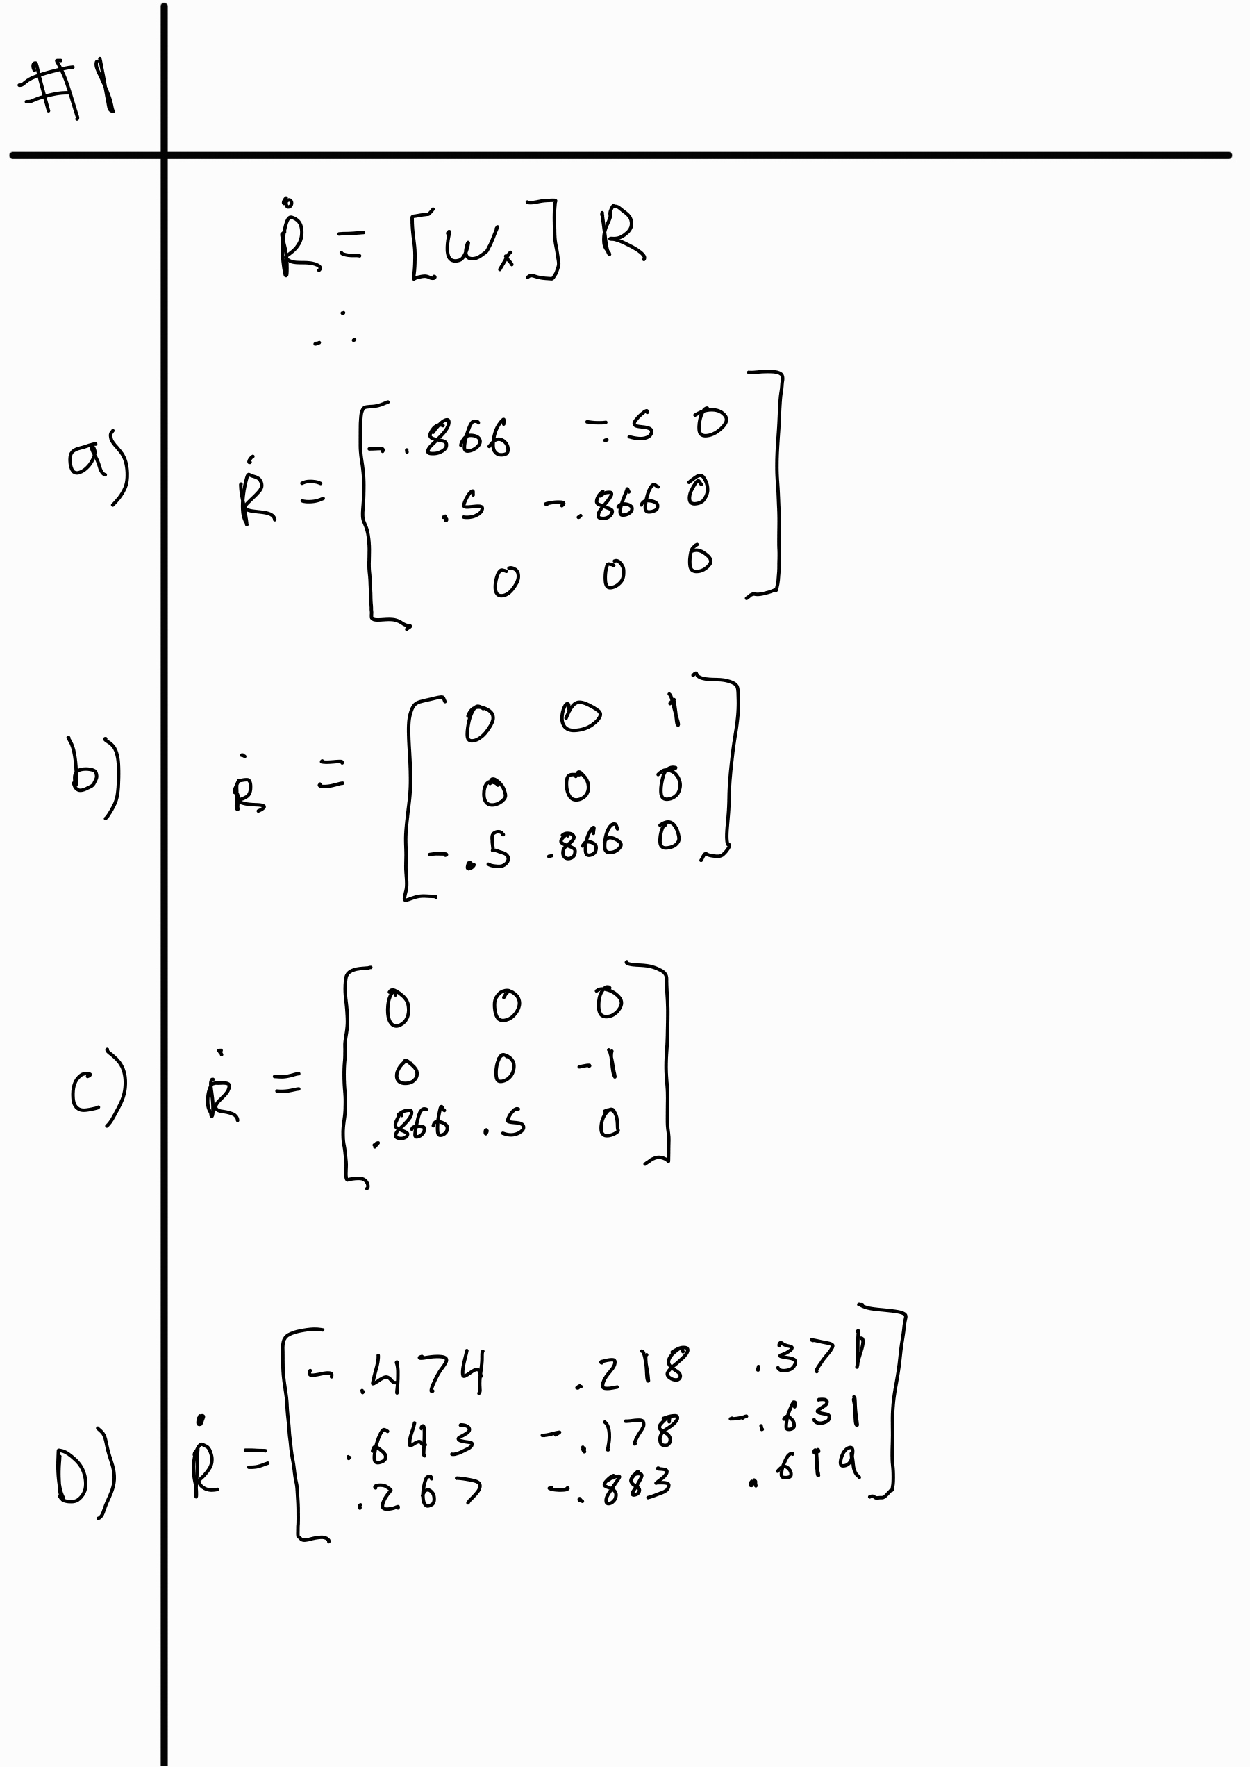
\includepdf[pages=-, pagecommand={\thispagestyle{plain}}, scale=0.9]{../Homework_7_hand_calcs.pdf}%
}{\noindent\textcolor{gray!60}{\itshape [Homework\_7\_hand\_calcs.pdf not yet added]}}

\end{document}
